% Created 2023-12-07 Thu 20:04
% Intended LaTeX compiler: pdflatex
\documentclass[12pt, a4paper]{article}
\usepackage[utf8]{inputenc}
\usepackage[T1]{fontenc}
\usepackage{graphicx}
\usepackage{longtable}
\usepackage{wrapfig}
\usepackage{rotating}
\usepackage[normalem]{ulem}
\usepackage{amsmath}
\usepackage{amssymb}
\usepackage{capt-of}
\usepackage{hyperref}
\usepackage{placeins}
\usepackage{gensymb}
\usepackage[letterpaper]{geometry}
\geometry{top=1.0in, bottom=1.0in, left=1.0in, right=1.0in}
\usepackage{rotating}
\usepackage{graphicx}
\usepackage{pgfplots}
\usepackage{filecontents}
\usepackage{tikz}
\usepackage{fancyhdr}
\usepackage{enumitem}
\pagestyle{fancy}
\lhead{}
\chead{}
\rhead{Johnson \thepage}
\lfoot{}
\cfoot{}
\rfoot{}
\renewcommand{\headrulewidth}{0pt}
\renewcommand{\footrulewidth}{0pt}
\setlength\headsep{0.333in}
\newcommand{\bibent}{\noindent \hangindent 40pt}
\newenvironment{workscited}{\newpage \begin{center} Works Cited \end{center}}{\newpage }
\graphicspath{ {./attachments/} }
\author{Christian}
\date{\today}
\title{}
\hypersetup{
 pdfauthor={Christian},
 pdftitle={},
 pdfkeywords={},
 pdfsubject={},
 pdfcreator={Emacs 28.2.50 (Org mode 9.7-pre)}, 
 pdflang={English}}
\begin{document}

\begin{document}
\begin{flushleft}
Christian Johnson\\
\vspace{2mm}Dr. Richard Hartnett\\
\vspace{2mm}Linear Circuits\\
\vspace{2mm}December 07 2023\\
\vspace{4mm}\begin{center}
Music Filtering Lab
\end{center}
\vspace{1mm}\setlength{\parindent}{0.5in}
\section*{Introduction}
\label{sec:org5baefae}
Filters are circuit components that are intended to amplify or mitigate certain frequencies or ranges of frequencies. They are used in many industries, particularly in sound design and music production. This lab sought to highlight these disciplines, presenting a practical learning experience in order to apply the concepts of filter design that this class has covered thus far to a popular industry. Presented with a partially corrupted sound file, the goal was to use existing knowledge of filter design to select a filter and its specifications in order to filter out the corrupted elements of the sound file.
\section*{Process}
\label{sec:org9c2dc21}
Upon opening the .wav file, there was a clearly evident chirping tone at a consistant frequency. Using MATLAB and the given code, I was able to generate several plots that provided more information about the file and its component frequencies. Shown below are a spectrogram, Fast Fourier Transform, and a Power Spectral Density plot.

\begin{figure}[!htb]
\minipage{0.32\textwidth}
  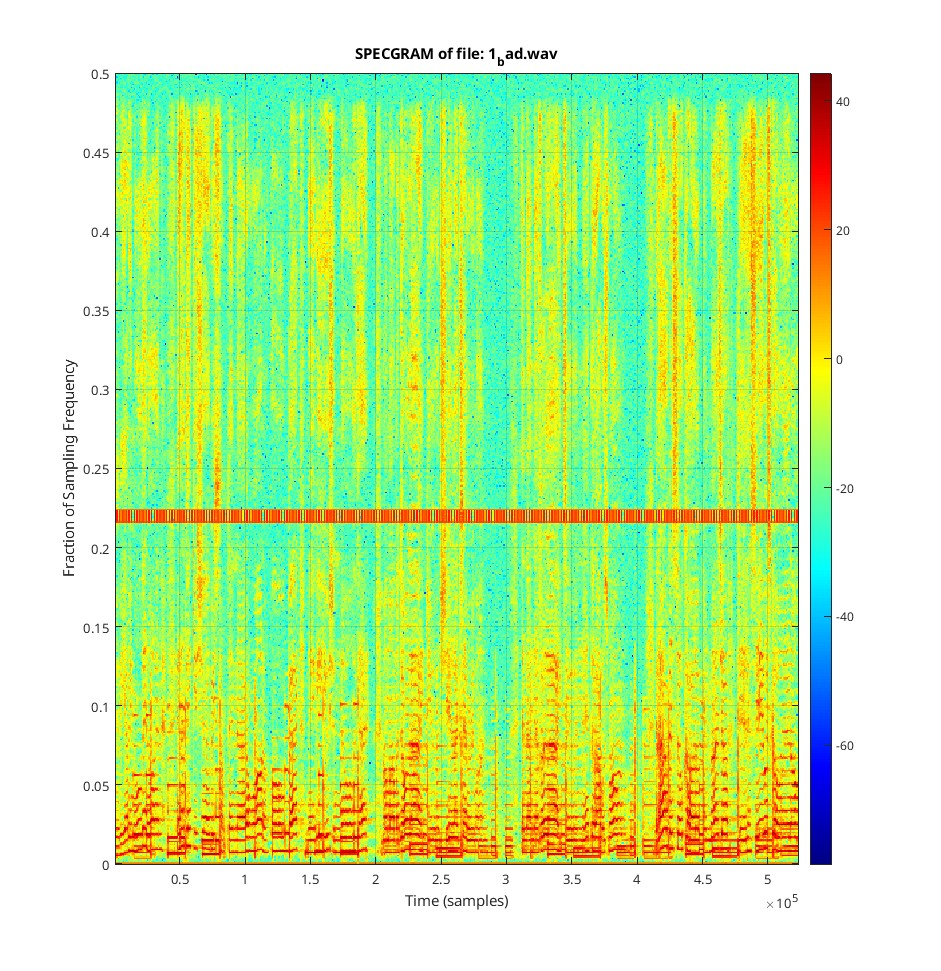
\includegraphics[width=\linewidth]{Pre-Spectrogram.jpg}
  \caption{Spectrogram}
\endminipage\hfill
\minipage{0.32\textwidth}
  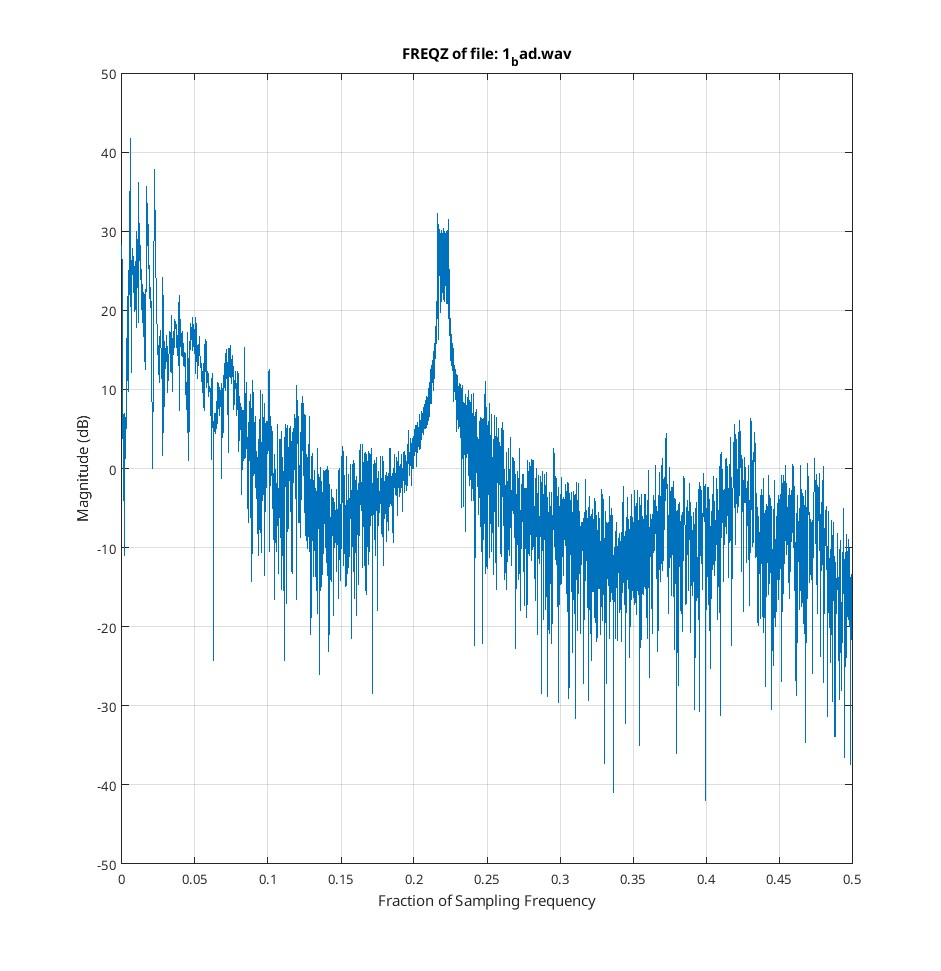
\includegraphics[width=\textwidth]{Pre-FFT.jpg}
  \caption{FFT}
\endminipage\hfill
\minipage{0.32\textwidth}
  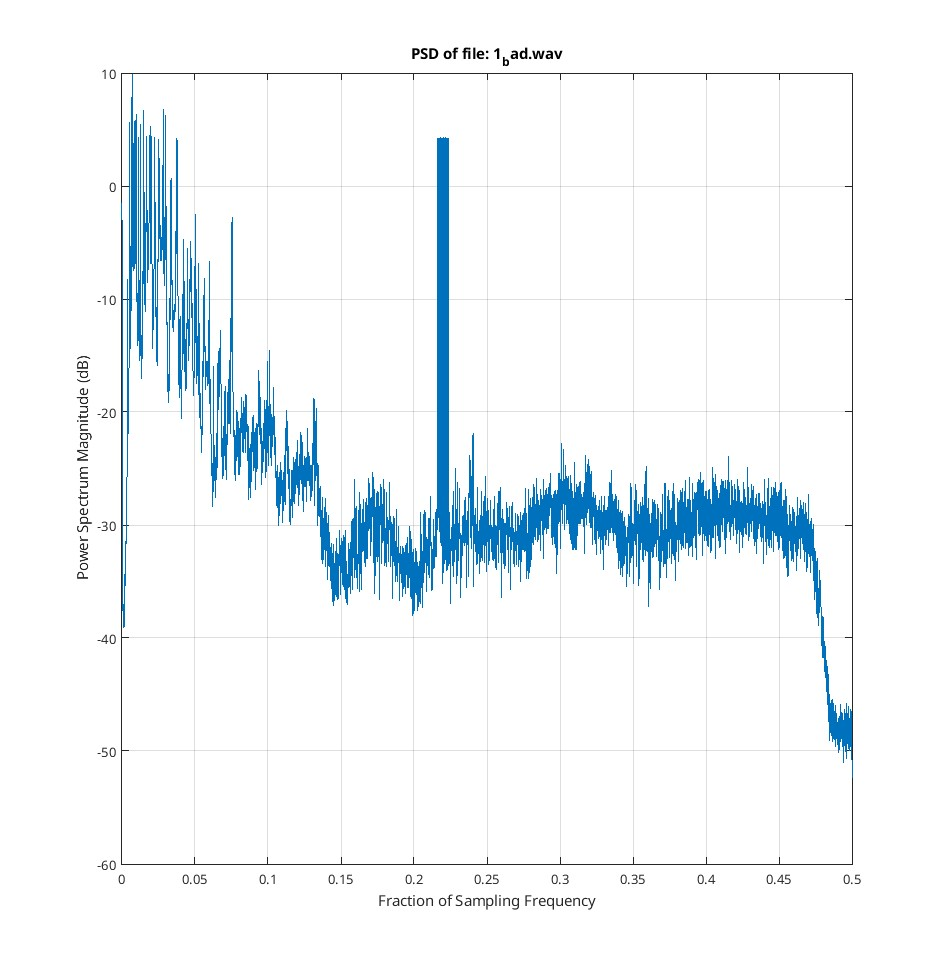
\includegraphics[width=\textwidth]{Pre-PSD.jpg}
  \caption{PSD}
\endminipage
\end{figure}

The spectrogram shows a reb bar across its width at about 0.23Fs. This red bar is a visual depiction of the errant frequencies in this file. Similarly, there is a visible peak in the FFT graph. This peak conveys very little usable information, but the FFT graph lets us find the PSD plot, which shows a clearly defined range of frequencies that stand out from the rest. These frequencies appear to range from 0.216Fs to 0.224Fs, extending about 35 dB above the rest of the signal. 
\section*{Design}
\label{sec:org15d40d6}
The PSD plot shows a discrete range of frequencies that are seperate from the rest of the waveform. This would indicate that a notch filter would perform best to attenuate these signals, since notch filters are intended to filter out very specific bands, leaving all else relatively untouched. In order to design a notch filter using the MATLAB code that I had previously written, I needed to find reasonable values for Amax, Amin, lower and upper passband, and lower and upper stopband. Amin represents the amount that I wish to attenuate the signals within the stopband. Since the errant frequencies extend about 35 dB above the highest point on the waveform, this seems like a reasonable value.  Amax represents the maximum allowance I am willing to give the filter in the passband, in other words, how much I am willing to allow the filter to alter frequencies outside of what I wish to filter. I chose 0.5 as an initial Amax, since I wished the passband to remain mostly unchanged, but I still needed to allow some freedom so that I wasn't attempting to model an ideal filter. The stopband limits deliminate the frequencies that I wish my notch filter to affect - I chose to set these as the limits of the frequency range in the PSD, 0.216Fs to 0.224Fs. From there I was able to choose initial values for my passband limits, which help to specify how tightly matched I wish the filters response to be to the stopband. The closer the passband limits are to the stopband, the better the filter will perform, but the higher the order will be. Since I was limited by an 8th order filter, it was necessary to balace filter performance with order through several trials, and I chose 0.2-0.23 as my initial values.

I was now able to run my design code with these values, calculating the transfer function for a digital notch butterworth filter with Amax of 0.5, Amin of 35, passband of 0.2-0.23, and stopband of 0.216-0.224. These values produced a 12th order filter, which told me that I needed to move my passband limits further away from my stopband. I adjusted the passband to 0.19-0.24, and produced an 8th order filter. The result produced a PSD which is shown below.

\begin{figure}[htb]
\minipage{0.5\textwidth}
\centering
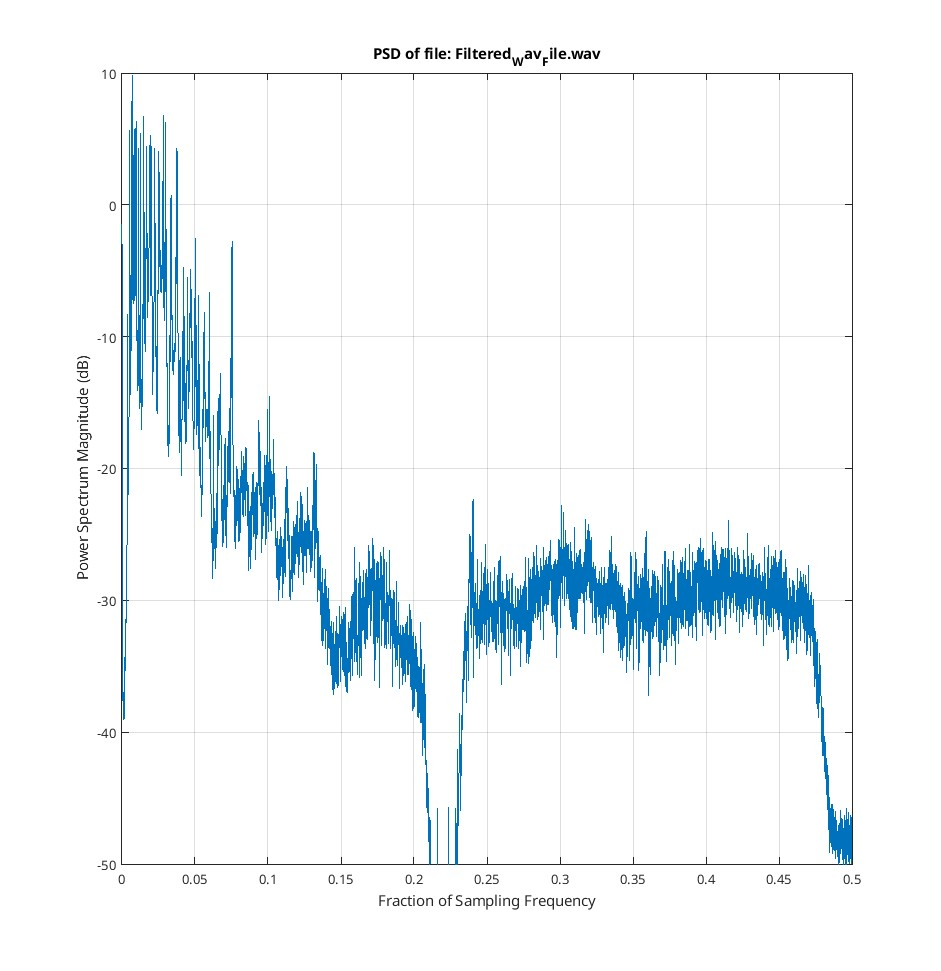
\includegraphics[width=0.5\linewidth]{Post-PSD.jpg}
\caption{PSD}
\endminipage
\minipage{0.5\textwidth}
\centering
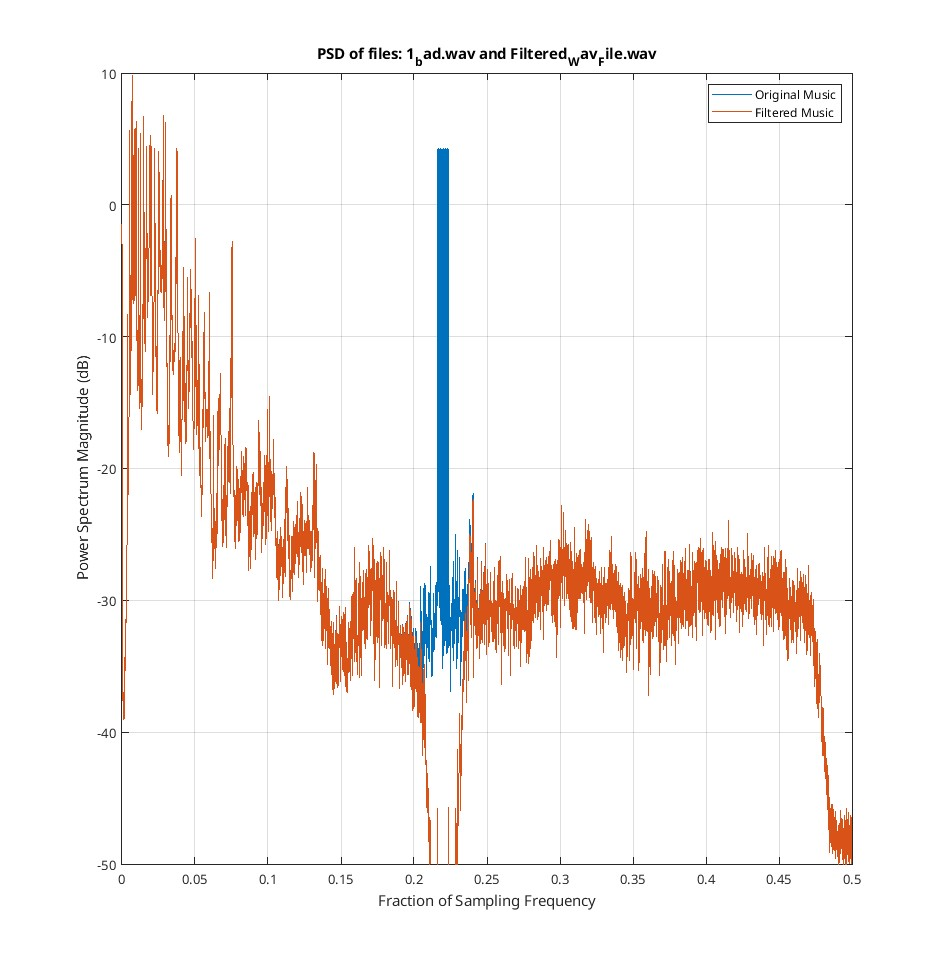
\includegraphics[width=0.5\linewidth]{Post-PSDOverlay.jpg}
\caption{PSD - Overlay}
\endminipage
\end{figure}

These figures show the PSD for the filtered music file, overlaid with the PSD from the original. The filtered plot completely removed the corrupted frequencies from the original file, with the remainder appearing to be relatively unchanged. Listening to the file itself affirms that the original music is in good condition, and all audible traces of the corruption have been removed. The working filter can be represented by the function:
\begin{center}
$H(z)=(\frac{z^{2}-0.3749z+1}{z^{2}-0.4107z+0.8383})(\frac{z^{2}-0.3749z+1}{z^{2}-0.2772z+0.8362})(\frac{z^{2}-0.3749z+1}{z^{2}-0.5268z+0.9308})(\frac{z^{2}-0.3749z+1}{z^{2}-0.1911z+0.9285})$
\end{center}
\newline
This transfer function can be represented graphically with the magnitude and pole/zero plots below.
\begin{figure}[!htb]
\minipage{0.5\textwidth}
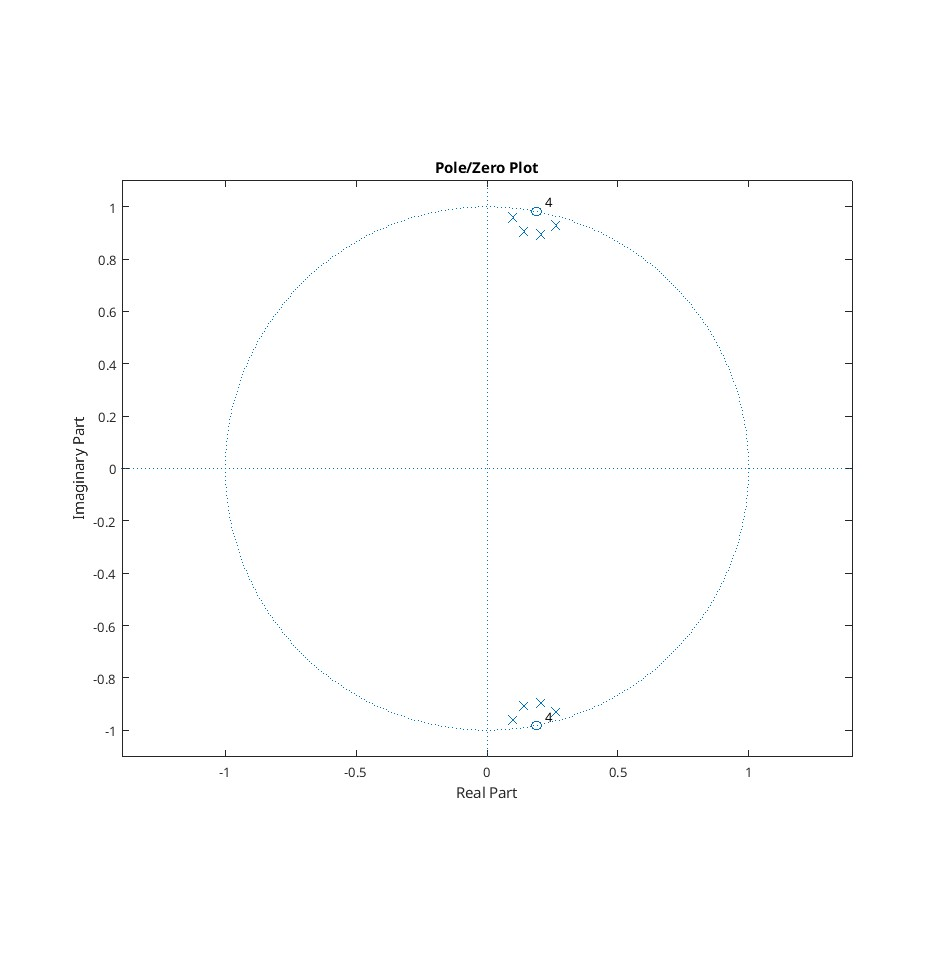
\includegraphics[width=\linewidth]{Pole-Zero.jpg}
\caption{Pole Zero Plot}
\endminipage
\minipage{0.5\textwidth}
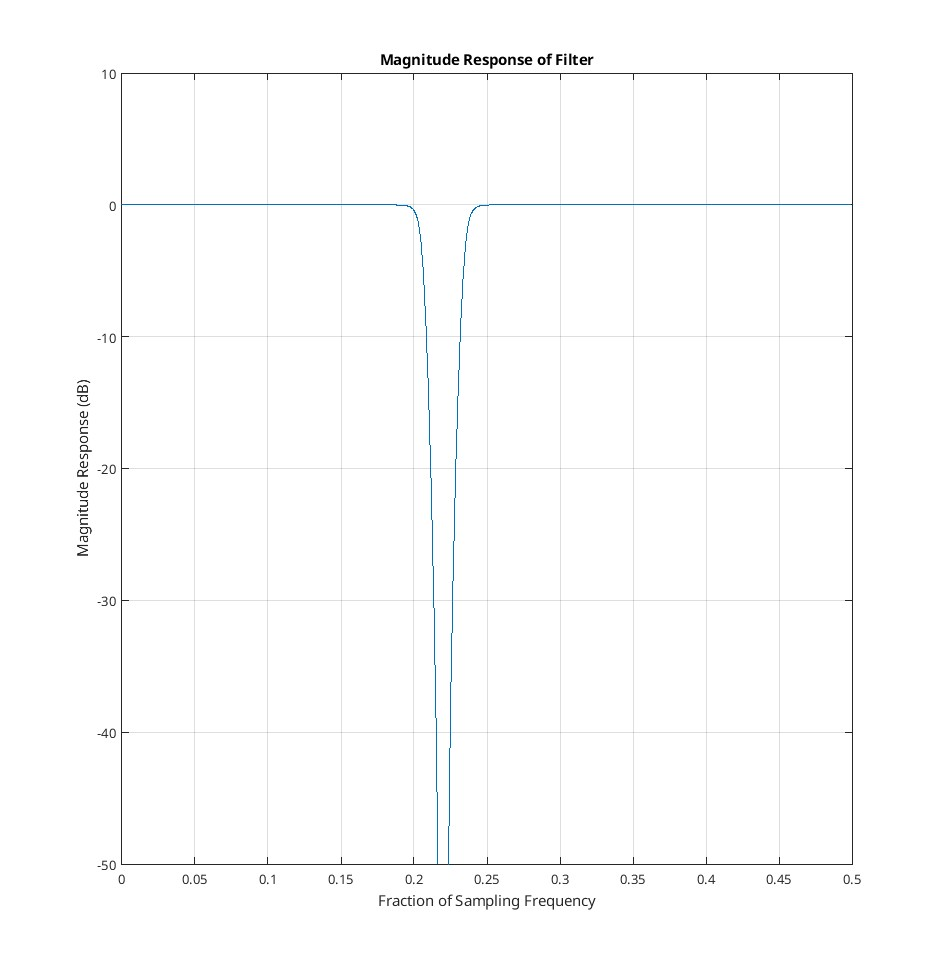
\includegraphics[width=\linewidth]{MagnitudeResponse.jpg}
\caption{Magnitude Plot}
\endminipage
\end{figure}
The designed notch filter performed extrememly well, precisely meeting the design requirements and removing the unwanted components from the corrupted music file. The PSD plots for the modified music files visually confirm this, displaying the difference between the modified and original files. The corrupted signals are no longer audible, and the original file seems largely unchanged outside of the expected range. This trial was an effective exploration into practical filter design, allowing us to better understand the specifications that we have been using all year and assign actual meaning to otherwise obscure variable names.  

\end{document}
\end{document}